\documentclass[11pt]{article}
\usepackage[a4paper,margin=2cm]{geometry}
\usepackage[T1]{fontenc}
\usepackage{lmodern}
\usepackage[protrusion=false,expansion=false]{microtype}
\DisableLigatures[-]{family=tt*}
\usepackage{booktabs}
\usepackage{array}
\usepackage{longtable}
\usepackage{graphicx}
\usepackage{amsmath}
\usepackage{amssymb}
\usepackage[hidelinks]{hyperref}
\usepackage{caption}
\captionsetup{font=small}
\usepackage{xcolor}
\usepackage{listings}
\usepackage{pifont}
\newcommand{\textbigstar}{\ding{72}}
\definecolor{codebg}{HTML}{F6F8FA}
\definecolor{codeframe}{HTML}{D0D7DE}
\definecolor{codekw}{HTML}{0550AE}
\definecolor{codestr}{HTML}{0A3069}
\definecolor{codecomment}{HTML}{6E7781}
\definecolor{codeemph}{HTML}{8250DF}
\definecolor{notebg}{HTML}{FFF8E5}
\definecolor{destmain}{HTML}{1F6FEB}
\definecolor{destsupp}{HTML}{2DA44E}
\definecolor{destnone}{HTML}{8C959F}
\lstdefinestyle{vepyr}{
  basicstyle=\ttfamily\small,
  keywordstyle=\color{codekw}\bfseries,
  emphstyle=\color{codeemph},
  stringstyle=\color{codestr},
  commentstyle=\color{codecomment}\itshape,
  backgroundcolor=\color{codebg},
  frame=single, rulecolor=\color{codeframe}, framesep=4pt,
  xleftmargin=4pt, xrightmargin=4pt,
  columns=fullflexible, keepspaces=true, upquote=true,
  showstringspaces=false, breaklines=true,
  aboveskip=8pt, belowskip=8pt,
}
\lstset{style=vepyr}
\lstdefinelanguage{shell}{
  emph={vepyr,bcftools,tabix,python,pip},
  sensitive=true, morecomment=[l]{\#}, morestring=[b]", morestring=[b]',
}
\emergencystretch=3em

% Destination tags: where each block is meant to go.
\newcommand{\dest}[3]{%
  \par\medskip\noindent{\setlength{\fboxrule}{0.6pt}\fcolorbox{#1}{#1!8}{%
  \parbox{\dimexpr\textwidth-2\fboxsep-2\fboxrule}{%
  \textbf{\textcolor{#1}{#2}}\quad\small #3}}}\par\medskip}
\newcommand{\FloatBarrier}{\clearpage}
\makeatletter\newcommand{\tabinput}[1]{\@@input #1 }\makeatother
\newcommand{\destmain}[1]{\dest{destmain}{$\rightarrow$ MAIN TEXT}{#1}}
\newcommand{\destsupp}[1]{\dest{destsupp}{$\rightarrow$ SUPPLEMENTARY}{#1}}
\newcommand{\destnone}[1]{\dest{destnone}{NOT FOR THE PAPER}{#1}}

\newcommand{\NVariants}{4{,}096{,}123}
\newcommand{\NManeRecords}{1{,}787{,}380}
\newcommand{\NPlof}{158}
\newcommand{\NHc}{57}
\newcommand{\NHcRare}{10}
\newcommand{\NHcCommon}{47}
\newcommand{\NHcHom}{12}
\newcommand{\NHcRareHom}{1}
\newcommand{\NHcGenes}{52}
\newcommand{\NFlagged}{100}
\newcommand{\NPlp}{1}
\newcommand{\NPlpHet}{1}
\newcommand{\NPlpHom}{0}
\newcommand{\NPlpArHet}{0}
\newcommand{\NBiallelic}{1}
\newcommand{\NManeGenes}{18{,}352}
\newcommand{\NManeGenesLtNinety}{1{,}134}
\newcommand{\NClinGenGenes}{2{,}302}
\newcommand{\NClinGenLtNinety}{83}
\newcommand{\NClinGenLtFifty}{19}
\newcommand{\NClinGenLtNinetySegdup}{8}
\newcommand{\NClinGenLtNinetyDifficult}{37}
\newcommand{\ClinGenFalseDup}{\textit{CBS}, \textit{ICOSLG}, \textit{PRODH}}
\newcommand{\AnnotateMin}{4.2}
\newcommand{\AnnotateSec}{255}
\newcommand{\Workers}{8}
\newcommand{\TierThreeMin}{0.6}
\newcommand{\AnalyzeMin}{1.3}
\newcommand{\VepyrVersion}{0.10.0}
\newcommand{\PolarsVersion}{1.44.2}
\newcommand{\PolarsBioVersion}{0.36.2}
\newcommand{\FlagLastExon}{55}
\newcommand{\FlagRefMinor}{13}
\newcommand{\FlagSpliceai}{3}
\newcommand{\FlagClinvarBenign}{39}
\newcommand{\FlagFiftybp}{4}
\newcommand{\FlagSegdup}{24}
\newcommand{\FlagLowmap}{10}
\newcommand{\LoeufSynN}{288}
\newcommand{\LoeufSynPct}{24.7}
\newcommand{\LoeufSynOr}{1.00}
\newcommand{\LoeufSynP}{1.000}
\newcommand{\LoeufSynMedian}{0.88}
\newcommand{\LoeufAmLbN}{351}
\newcommand{\LoeufAmLbPct}{15.7}
\newcommand{\LoeufAmLbOr}{0.57}
\newcommand{\LoeufAmLbP}{0.005}
\newcommand{\LoeufAmLbMedian}{1.00}
\newcommand{\LoeufAmLpN}{47}
\newcommand{\LoeufAmLpPct}{19.1}
\newcommand{\LoeufAmLpOr}{0.72}
\newcommand{\LoeufAmLpP}{0.466}
\newcommand{\LoeufAmLpMedian}{1.01}
\newcommand{\LoeufAllPlofN}{126}
\newcommand{\LoeufAllPlofPct}{9.5}
\newcommand{\LoeufAllPlofOr}{0.32}
\newcommand{\LoeufAllPlofP}{2.9\times10^{-4}}
\newcommand{\LoeufAllPlofMedian}{1.22}
\newcommand{\LoeufHcCommonN}{36}
\newcommand{\LoeufHcCommonPct}{13.9}
\newcommand{\LoeufHcCommonOr}{0.49}
\newcommand{\LoeufHcCommonP}{0.210}
\newcommand{\LoeufHcCommonMedian}{1.12}
\newcommand{\LoeufHcRareN}{9}
\newcommand{\LoeufHcRarePct}{0.0}
\newcommand{\LoeufHcRareOr}{0.00}
\newcommand{\LoeufHcRareP}{0.121}
\newcommand{\LoeufHcRareMedian}{0.95}
\newcommand{\LoeufFlaggedN}{80}
\newcommand{\LoeufFlaggedPct}{8.8}
\newcommand{\LoeufFlaggedOr}{0.29}
\newcommand{\LoeufFlaggedP}{0.002}
\newcommand{\LoeufFlaggedMedian}{1.24}
\newcommand{\NCoding}{20{,}725}
\newcommand{\NAfterTierOne}{94}
\newcommand{\NAfterTierTwo}{68}
\newcommand{\NAfterTierThree}{57}
\newcommand{\NRemoteSources}{12}
\newcommand{\RemoteSec}{57}
\newcommand{\RemoteRows}{25.9}
\newcommand{\NRareAsjCommon}{4}
\newcommand{\NRareMaternal}{5}
\newcommand{\NRarePaternal}{3}
\newcommand{\PlpGene}{F11}
\newcommand{\PlpHgvsp}{p.Glu135Ter}
\newcommand{\PlpAf}{0.063}
\newcommand{\PlpAsj}{1.85}
\newcommand{\PlpFold}{29}
\newcommand{\PlpParent}{father}


\title{Three tiers of annotation in a whole genome:\\
the GIAB HG002 case study\\[4pt]
\large Working document: biological story, main-text fragments,
Figure~1D and a Supplementary Data section}
\author{vepyr paper}
\date{\today}

\begin{document}
\maketitle

\noindent\colorbox{notebg}{\parbox{\dimexpr\textwidth-2\fboxsep}{\small
\textbf{How to read this document.} Each block is tagged with its intended
destination:
\textcolor{destmain}{\textbf{MAIN TEXT}} (Results, Discussion, Figure~1D),
\textcolor{destsupp}{\textbf{SUPPLEMENTARY}} (a complete section that can be
moved into \texttt{vepyr-supplementary.tex}) or
\textcolor{destnone}{\textbf{NOT FOR THE PAPER}} (the story for the authors
and notes on the analysis). Draft on branch
\texttt{paper/hg002-tiered-annotation}, not merged. Every number is generated
from the analysis outputs (\texttt{analysis.py} $\rightarrow$
\texttt{results/} $\rightarrow$ \texttt{make\_tex.py}); rerunning the
analysis updates text, tables and figures together.}}

\tableofcontents

%% ===================================================================
\clearpage
\section{The biological story}
\label{sec:story}
\destnone{Background for the authors; the paper uses the condensed
fragments of Sections~\ref{sec:results}--\ref{sec:fig1}.}
\paragraph{Why HG002.} HG002 (NA24385) is the son in the Ashkenazi Jewish
trio of the Genome in a Bottle consortium, a Personal Genome Project
participant with open consent and the most thoroughly characterised human
genome~\cite{zook2016,wagner2022}. Three properties make it a good test bed
for an annotation paper: a curated benchmark call set
(\NVariants{} small variants on chromosomes 1--22 after decomposition) with
explicit benchmark regions; matching benchmark VCFs for both parents
(HG003, HG004), which allow inheritance to be checked; and a founder
population, in which global allele frequencies can be misleading. The
question we ask is the classic one of MacArthur et
al.~\cite{macarthur2012}: \emph{how many genes does a healthy person knock
out, which of these calls are real, and what does this genome carry that a
clinician would care about?} Each step of the answer needs a different kind
of annotation, which is the point of the vepyr design.

\paragraph{1. A healthy genome carries tens of real LoF variants, and many
more false ones.} The core annotation finds \NPlof{} variants with a pLoF
consequence (stop-gained, frameshift, canonical splice site) in a MANE
Select transcript~\cite{morales2022}. Filters in the spirit of
LOFTEE~\cite{karczewski2020} reduce them to \NHc{} high-confidence pLoF
variants in \NHcGenes{} genes, \NHcHom{} of them homozygous, in line with
earlier estimates of about a hundred LoF variants and about twenty
homozygous LoF genes per genome~\cite{macarthur2012}, given that our counts
are restricted to MANE transcripts and benchmark regions. The removed calls
form recognisable classes, and each class comes from a different tier:
\begin{itemize}
\item \emph{Tier 1 (core cache).} \FlagLastExon{} premature stops in the
  last exon, which escape nonsense-mediated decay. \FlagRefMinor{} calls
  where the ``LoF'' allele is near-fixed in gnomAD: pairs of nearby
  frameshifts in \textit{SON} and \textit{SLAIN1} that restore the reading
  frame (GRCh38 carries a rare sequence there), and \textit{FMO2}
  p.Gln472Ter, the \textit{FMO2*2} allele that truncates FMO2 in most
  humans~\cite{dolphin1998}---a real, but species-wide, loss.
\item \emph{Tier 2 (plugins).} \FlagClinvarBenign{} variants classified
  benign in ClinVar, including \textit{LPL} p.Ser474Ter (S447X), a stop-gain
  associated with lower triglycerides~\cite{rip2006}, and the
  \textit{CYP2D6*4} splice-acceptor allele, a genuine loss of function in a
  pharmacogene that ClinVar classifies as a drug-response allele.
  \FlagSpliceai{} canonical splice-site variants without SpliceAI
  support~\cite{jaganathan2019}.
\item \emph{Tier 3 (ad hoc).} \FlagSegdup{} calls in segmental duplications
  (olfactory receptors, \textit{NBPF}, \textit{GOLGA8}, \textit{NPIPB},
  \textit{CYP2D6}) and \FlagLowmap{} in low-mappability regions, from GIAB
  stratifications~\cite{dwarshuis2024}; \FlagFiftybp{} premature stops within
  50\,bp of the last exon junction, from Ensembl exon coordinates.
\end{itemize}

\paragraph{2. Purifying selection is visible in one genome.} Joining the
frame with gnomAD v4.1 gene constraint (read from the gnomAD bucket by URL)
shows that only \LoeufAllPlofPct\% of HG002 pLoF variants fall in the 20\%
most LoF-intolerant genes, against \LoeufSynPct\% of rare synonymous variants
($p=\LoeufAllPlofP$), and none of the rare high-confidence ones does. A
healthy individual carries LoF variants, but in genes that tolerate them.
The rare synonymous reference matters: constrained genes are longer, so a
naive uniform expectation (20\%) would understate the depletion.

\paragraph{3. One clinically classified variant: an Ashkenazi founder
allele.} The only ClinVar pathogenic or likely pathogenic variant with
review criteria is \textit{F11} \PlpHgvsp{}, the factor~XI ``type~II''
allele (Glu117Ter in legacy numbering), one of the two founder mutations
that account for most factor~XI deficiency in Ashkenazi
Jews~\cite{asakai1991}. HG002 is heterozygous; the allele was transmitted
by the \PlpParent{}; its gnomAD frequency is \PlpAf\% overall but \PlpAsj\%
in Ashkenazi Jewish samples (\PlpFold-fold). The same founder effect shows
across the rare pLoF variants: \NRareAsjCommon{} of the \NHcRare{} that are
rare in gnomAD overall exceed 1\% in Ashkenazi Jewish samples, so
``rare'' depends on the reference population. Population-specific
frequencies come from the core cache; ClinVar from a plugin cache; the
parental genotypes from the parents' VCFs streamed from S3.

\paragraph{4. The trio resolves origins and exposes one false homozygous
LoF.} Nine of the ten rare high-confidence pLoF variants have a resolved
origin (\NRareMaternal{} maternal, \NRarePaternal{} paternal, one carried by
both parents) and none is a candidate \emph{de novo} variant. The one
homozygous rare pLoF, a 45-bp deletion of the canonical exon~2 donor of
\textit{PEX5}, would imply Zellweger spectrum disorder if it were a loss of
function. Both parents are homozygous for it, which already argues against
rarity (ClinVar classifications of the deletion are conflicting), and the exon has an alternative donor 45\,bp downstream that keeps
the reading frame. Absence from gnomAD here reflects the length of the
deletion, not its frequency. The case is a useful reminder that
transcript-level LoF calls need biological context; in this analysis the
context comes from the ad hoc tier.

\paragraph{5. What this genome cannot tell us.} Interval coverage of MANE
coding sequence by the benchmark regions shows that \NClinGenLtNinety{}
ClinGen disease genes~\cite{strande2017} are less than 90\% assessable in
HG002 v4.2.1, \NClinGenLtFifty{} less than half. They include genes in
segmental duplications and falsely duplicated regions of GRCh38
(\ClinGenFalseDup{}; \textit{CBS}, classic homocystinuria, is a known
example~\cite{aganezov2022}), \textit{FXN} (Friedreich ataxia) and GC-rich
genes such as \textit{ETFB}, \textit{GNPTG} and \textit{FAM20C}. Finding no
pathogenic variant in these genes is not evidence of absence.

\paragraph{Why this belongs in the vepyr paper.} The analysis is a single
Python session: \AnnotateMin\,min of annotation of the whole genome with
VEP-identical core fields and four plugins, then \AnalyzeMin\,min for
everything else, including \RemoteSec\,s to read \NRemoteSources{} remote
sources (\RemoteRows{} million records) without downloading, indexing or
converting them. Three kinds of annotation with three update rates---Ensembl
releases, ClinVar weeks, per-question data---are handled by three
mechanisms: a core cache, plugin caches and DataFrame operations on data read
from URLs. The biology is not new, which is the point: a known result
(depletion of LoF from constrained genes), a known founder allele and a
known reference artefact are recovered quickly, reproducibly and in one
place, which is what users need when the question, not the method, is new.


%% ===================================================================
\clearpage
\section{Main text: Results fragment}
\label{sec:results}
\destmain{Results, new subsection after ``Performance tests'' (or as the
``Annotation with analytical workflows'' item of the Results outline).
About 290 words; can be cut to the first three sentences and the F11 sentence.}
\subsection*{Three tiers of annotation in a whole genome}
% Suggested heading; numbers below are from the analysis outputs.

To show how annotation that changes at different rates is combined in one
analysis, we annotated the GIAB HG002 benchmark call set (\NVariants{}
variants, chromosomes 1--22) with the Ensembl~116 core cache and four plugin
caches (ClinVar, SpliceAI, AlphaMissense and CADD) in
\AnnotateMin\,min on a laptop, and joined the resulting frame with
\NRemoteSources{} sources that were read directly from their URLs by
polars-bio and Polars: gnomAD gene constraint, ClinGen gene--disease
validity, Ensembl gene models, GIAB genome stratifications and benchmark
regions, and the benchmark VCFs of both parents (Figure~1D; Supplementary
Section~X). Of \NPlof{} variants with a predicted loss-of-function (pLoF)
consequence in a MANE Select transcript, filters drawn from the three
tiers---escape from nonsense-mediated decay and near-fixed alleles (core
cache), SpliceAI and ClinVar (plugins), and segmental duplications, low
mappability and the 50-bp rule (ad hoc sources)---retained \NHc{}
high-confidence pLoF variants in \NHcGenes{} genes. pLoF variants were
depleted from LoF-intolerant genes (\LoeufAllPlofPct\% vs \LoeufSynPct\% of
rare synonymous variants in the two lowest LOEUF deciles,
$p=\LoeufAllPlofP$), the signature of purifying selection in a single
genome. The only pathogenic ClinVar variant with review criteria was the
Ashkenazi founder allele \textit{\PlpGene} \PlpHgvsp{}, heterozygous and
inherited from the \PlpParent{}, with a frequency of \PlpAsj\% in Ashkenazi
Jewish gnomAD samples. Interval coverage showed that \NClinGenLtNinety{} of
\NClinGenGenes{} ClinGen genes have less than 90\% of their coding sequence
within the benchmark regions, including \textit{CBS}, which lies in a
falsely duplicated region of GRCh38. The ad hoc sources were read in
\RemoteSec\,s, and the analysis after annotation took \AnalyzeMin\,min.


\section{Main text: Discussion / Conclusion fragment}
\label{sec:discussion}
\destmain{Conclusion (\texttt{vepyr-main.tex}, ``The \emph{vepyr} \ldots'';
matches the ``recurrent vs.\ ad hoc analysis'' note there). About 120 words.}
The HG002 example separates annotation by how often it changes rather than
by where it comes from. Core annotation follows Ensembl releases and plugin
data follow their providers; both are compiled once into indexed Parquet
caches, so a weekly ClinVar release rebuilds a 0.1\,GiB plugin cache, not
the core cache. Data that a particular question needs---gene constraint,
curated gene--disease relationships, genome stratifications or the genotypes
of relatives---need no cache at all: they are read from their URLs when the
query runs and combined with the annotation through joins and interval
operations. In a VEP-based workflow, each such source is configured as a
custom annotation or plugin before annotation, or processed afterwards from
an annotated VCF with separate tools. Keeping the third tier outside the
annotation engine lets analyses change without changing, or re-running,
the annotation.


%% ===================================================================
\clearpage
\section{Main text: Figure 1D}
\label{sec:fig1}
\destmain{Figure~1, panel~D, replacing the chromosome~22 ``Beyond
\texttt{filter\_vep}'' panel; generated by
\nolinkurl{paper/figure1/build_tiered_annotation.py}.}
The panel below replaces the current panel~D (``Beyond \texttt{filter\_vep}'',
chromosome~22, segmental duplications) of the cache-workflow version of
Figure~1. It is generated by \nolinkurl{paper/figure1/build_tiered_annotation.py}
in the same draw.io/SVG style as the other panels and reads its numbers from
\texttt{results/}. The chromosome~22 segmental-duplication example can stay
in the supplement as the bedtools-verified equivalence check.

\begin{figure}[ht]
\centering
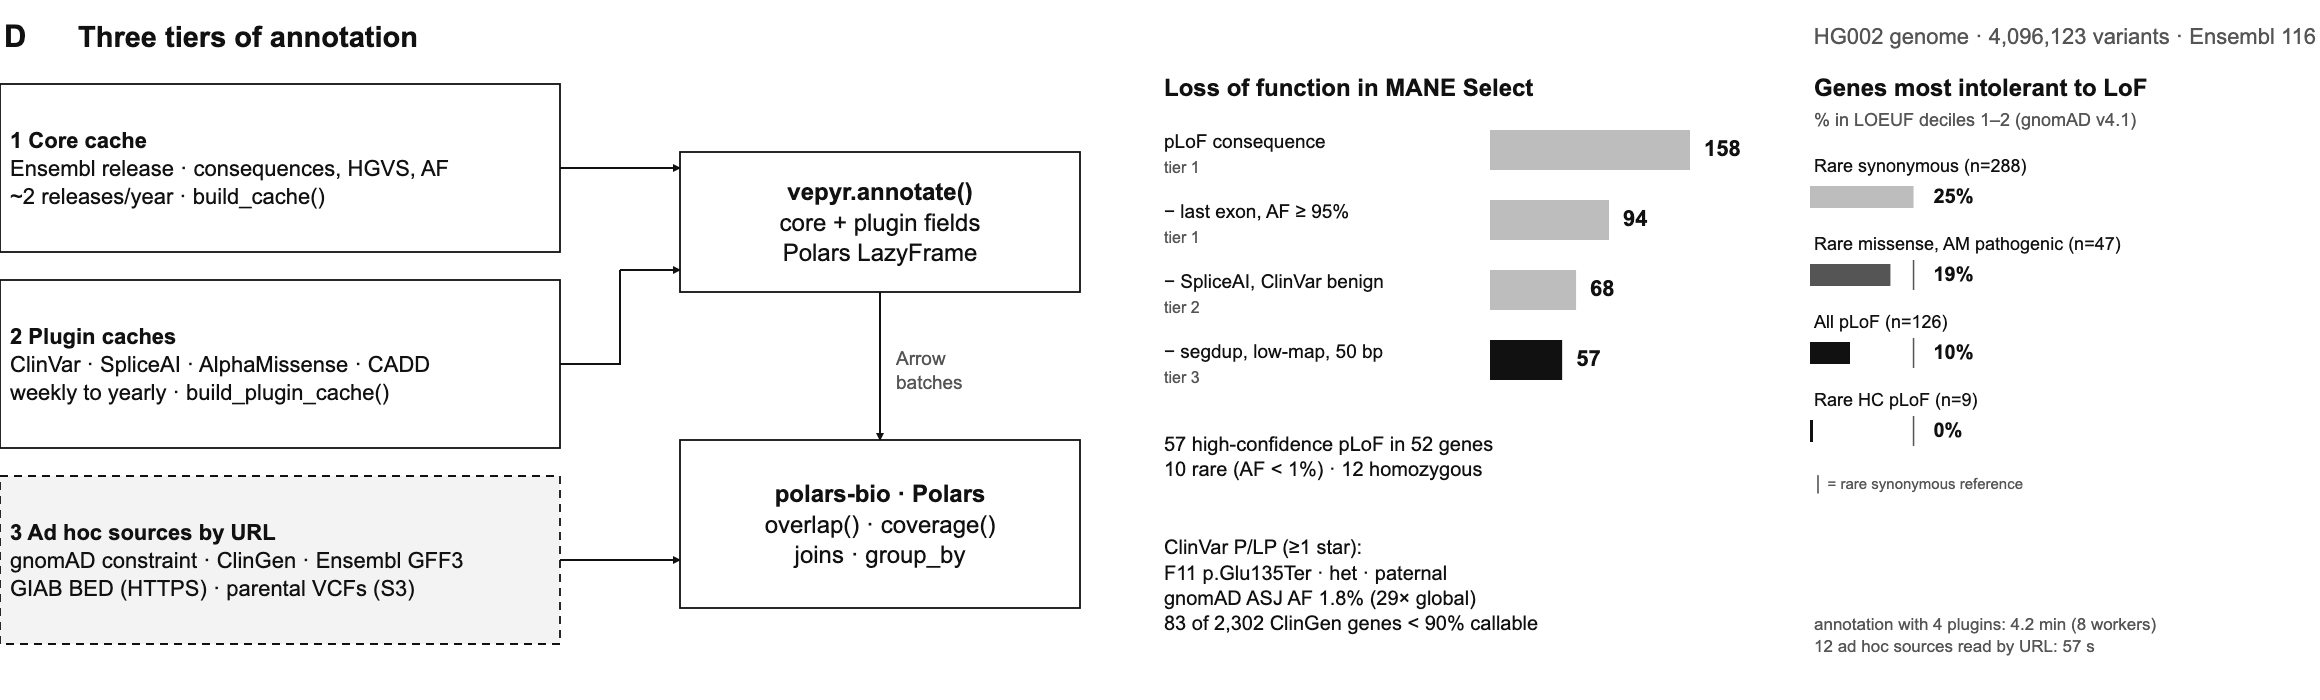
\includegraphics[width=\textwidth]{../figure1/d-tiered-annotation-proposal.png}
\caption*{\textbf{Figure 1D (proposal). Three tiers of annotation in the HG002
genome.} Core (tier~1) and plugin (tier~2) annotations are produced by
\texttt{vepyr.annotate()} from prebuilt Parquet caches that are refreshed at
different rates; ad hoc sources (tier~3) are read directly from their URLs by
polars-bio and Polars when the query runs and are combined with the annotated
frame by joins and interval operations (\texttt{overlap()},
\texttt{coverage()}). Middle: variants with a predicted loss-of-function
(pLoF) consequence in a MANE Select transcript that remain after the filters
contributed by each tier (last exon; SpliceAI support and ClinVar benign
classification; segmental duplications, low mappability and the 50-bp rule),
leaving \NHc{} high-confidence pLoF variants in \NHcGenes{} genes. Right:
share of each variant class in the 20\% of genes most intolerant to LoF
(gnomAD v4.1 LOEUF deciles 1--2); ticks mark the share of rare synonymous
variants. pLoF variants are depleted from these genes, as expected under
purifying selection. Bottom of the middle column: the only ClinVar
pathogenic variant with review criteria, the Ashkenazi founder allele
\textit{F11} \PlpHgvsp{}, with its parental origin from the parental VCFs,
and the number of ClinGen genes with less than 90\% of their coding sequence
in the benchmark regions. Details in Supplementary Section~X.}
\end{figure}

\begin{figure}[p]
\centering
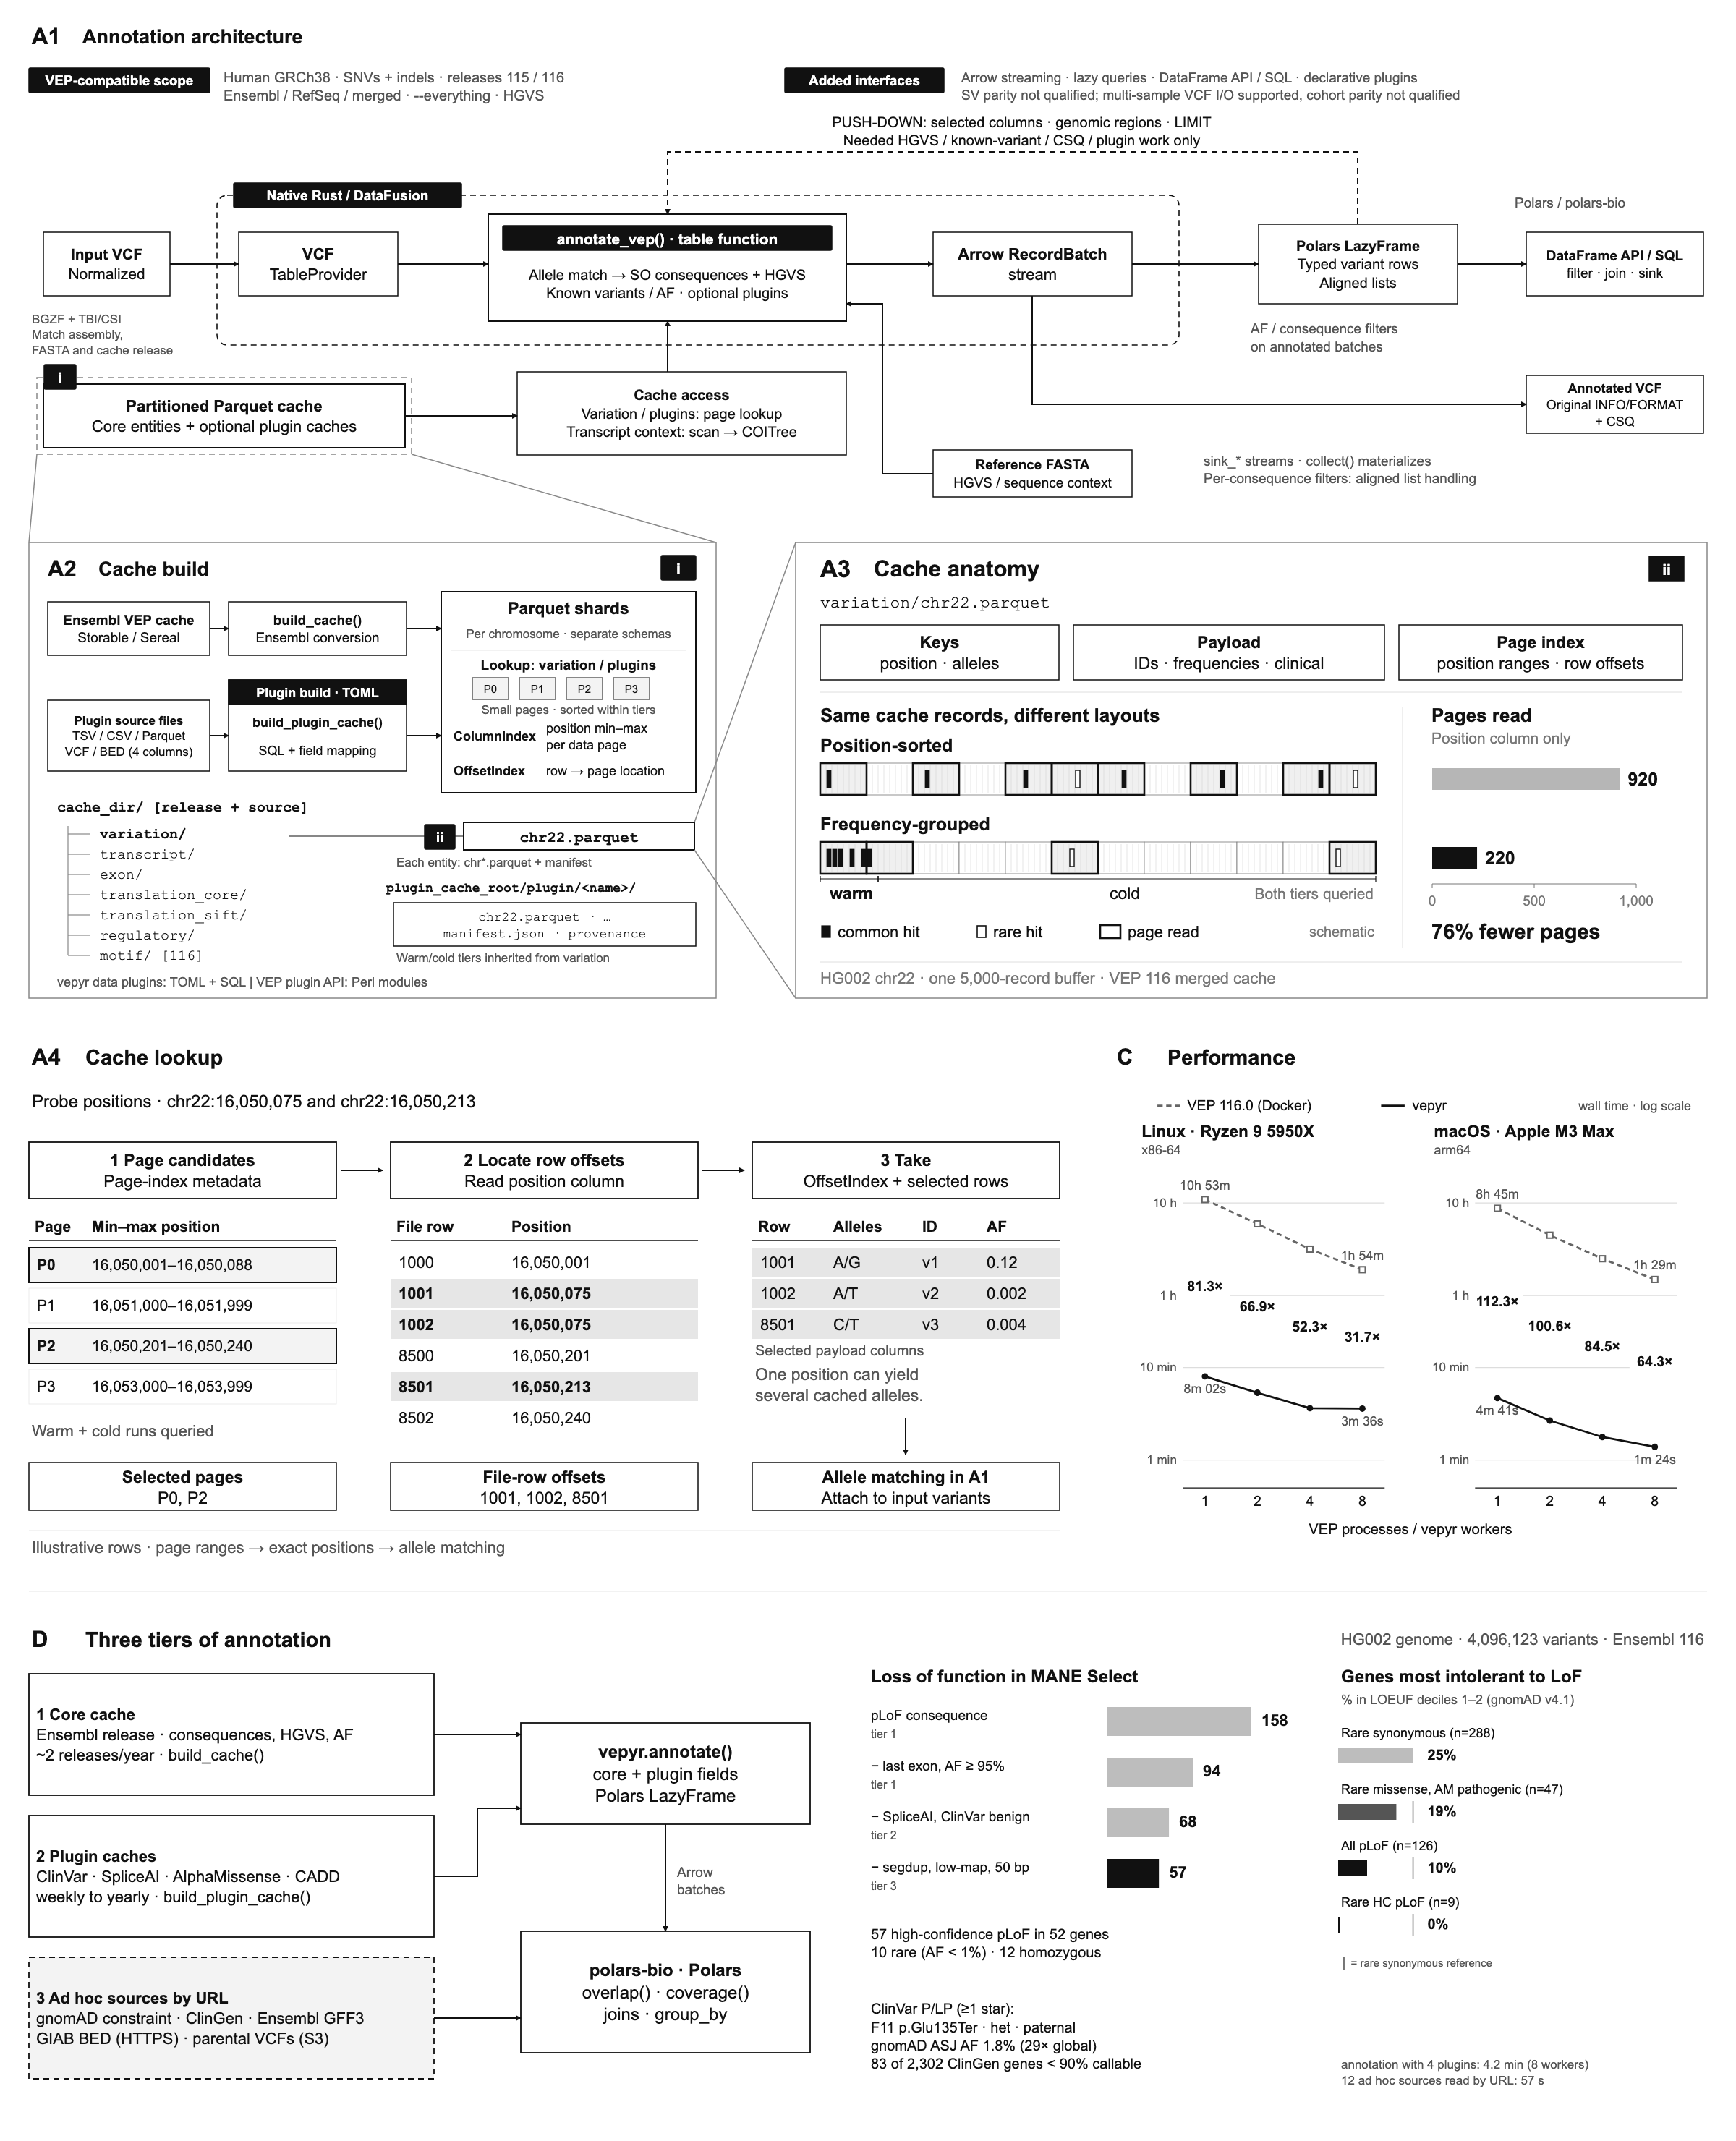
\includegraphics[width=\textwidth]{../figure1/figure1-tiered-annotation-proposal.png}
\caption*{Figure~1 (cache-workflow proposal) with the new panel~D in place of
the previous one, for checking proportions. Panels A1--A4 and C are
unchanged.}
\end{figure}


%% ===================================================================
\clearpage
\section{Supplementary section: three tiers of annotation in the HG002 genome}
\label{sec:supp}
\destsupp{New section of \texttt{vepyr-supplementary.tex}, after
``Beyond \texttt{filter\_vep}: interval operations''. Self-contained:
methods, code, figures, tables.}
Annotation sources change at different rates. The Ensembl core annotation
(transcript models, consequences, HGVS, known variants and population
frequencies) changes with Ensembl releases, about twice a year; resources
such as ClinVar change weekly, and prediction scores (SpliceAI,
AlphaMissense, CADD) with new model releases; and many questions need data
that are not annotation sources at all: gene-level constraint, curated
gene--disease relationships, gene models, genome stratifications or the
genotypes of relatives. vepyr maps the first two onto prebuilt Parquet caches
(tiers~1 and~2 below) and leaves the third to the DataFrame ecosystem: such
sources are read when a query needs them, directly from their URLs, without
a build step (Table~\ref{tab:tiers}).

\begin{table}[ht]
\centering\small
\begin{tabular}{p{0.15\textwidth}p{0.29\textwidth}p{0.17\textwidth}p{0.3\textwidth}}
\toprule
Tier & Sources used here & Changes & Mechanism \\
\midrule
1 Core cache & Ensembl~116 \texttt{ensembl} cache: consequences, HGVS, MANE, gnomAD frequencies & with Ensembl releases (about twice a year) & \texttt{build\_cache()}; Parquet; read during annotation \\
2 Plugin caches & ClinVar (2026-07-06), SpliceAI, AlphaMissense, CADD~v1.7 & weekly (ClinVar) to yearly & \texttt{build\_plugin\_cache()} from TOML manifests; Parquet; matched during annotation \\
3 Ad hoc sources & gnomAD~v4.1 constraint, ClinGen gene validity, Ensembl~116 GFF3, GIAB v3.6 stratifications, GIAB v4.2.1 benchmark regions and parental VCFs & per analysis & read from the URL by polars-bio or Polars when the query runs; joins and interval operations \\
\bottomrule
\end{tabular}
\caption{The three tiers of annotation used in this section.}
\label{tab:tiers}
\end{table}

The example combines the three tiers in one analysis of the GIAB HG002
genome: which predicted loss-of-function (pLoF) variants does a healthy
individual carry, does purifying selection against them show in a single
genome, which clinically classified variants does HG002 carry and from which
parent, and in which clinically relevant genes would a negative result be
uninformative because the gene lies outside the benchmark regions?

\subsection{Data and software}
The input is the NIST v4.2.1 GRCh38 benchmark call set of HG002
(chromosomes 1--22), with multi-allelic records decomposed as in the quick
start, which yields \NVariants{} records. The analysis used the
\texttt{ensembl} core cache of release~116, the ClinVar, AlphaMissense,
SpliceAI and CADD plugin caches (chromosomes 1--22 only: 30\,GiB and
90\,GiB on disk), the Ensembl primary-assembly FASTA, vepyr~\VepyrVersion{},
Polars~\PolarsVersion{} and polars-bio~\PolarsBioVersion{} on an Apple
MacBook Pro (M3 Max, 64\,GiB). The ad hoc sources are listed in
Table~\ref{tab:adhoc}; none is stored locally.

\begin{lstlisting}[language=shell]
python -m venv hg002 && . hg002/bin/activate
pip install "vepyr[polars-bio]==0.10.0" scipy matplotlib
CHR=$(for c in $(seq 1 22); do printf -- "--chrom %s " $c; done)
vepyr download-cache --release 116 --cache_type ensembl --dir_cache vepyr_cache $CHR
for p in clinvar alphamissense spliceai cadd; do
  vepyr download-plugin-cache --plugin $p --release 116 \
    --plugin_cache_root vepyr_plugin_cache $CHR
done
bcftools norm -m -both -Oz -o HG002_v4.2.1.split.vcf.gz \
  HG002_GRCh38_1_22_v4.2.1_benchmark.vcf.gz
tabix -p vcf HG002_v4.2.1.split.vcf.gz      # 4096123 records
\end{lstlisting}

\subsection{Tiers 1 and 2: annotation}
Core and plugin fields are produced by a single call. The annotated frame,
restricted to the 33 columns used later (including the gnomAD Ashkenazi
Jewish frequencies \texttt{gnomADe\_ASJ\_AF} and \texttt{gnomADg\_ASJ\_AF},
since HG002 is of Ashkenazi Jewish ancestry), is written once to Parquet; the
per-consequence fields remain aligned lists:
\begin{lstlisting}[language=Python]
import polars as pl
import polars_bio as pb
import vepyr

lf = vepyr.annotate(
    "HG002_v4.2.1.split.vcf.gz",
    "vepyr_cache/116_GRCh38_ensembl",
    reference_fasta="Homo_sapiens.GRCh38.dna.primary_assembly.fa",
    workers=8,
    plugin_cache_root="vepyr_plugin_cache",
    plugins=["clinvar", "alphamissense", "spliceai", "cadd"],
)
lf.select(*VARIANT_COLS, *CSQ_COLS).sink_parquet("HG002.annotated.parquet")
\end{lstlisting}
\noindent Annotation of the \NVariants{} records with the four plugins took
\AnnotateSec{}\,s (\AnnotateMin{}\,min) with \Workers{} workers.

\subsection{Tier 3: ad hoc sources read from their URLs}
Twelve sources are read (Table~\ref{tab:adhoc}). Interval sources are read with polars-bio, which converts BED to 1-based
closed coordinates, matching the vepyr frame; the parental VCFs are streamed
from the GIAB mirror on Amazon S3. Tabular gene-level sources and the GFF3
gene models are read with Polars:
\begin{lstlisting}[language=Python]
GIAB = "https://ftp-trace.ncbi.nlm.nih.gov/ReferenceSamples/giab/release"
STRAT = f"{GIAB}/genome-stratifications/v3.6/GRCh38@all"
segdups = pb.scan_bed(f"{STRAT}/SegmentalDuplications/GRCh38_segdups.bed.gz")
benchmark = pb.scan_bed(f"{GIAB}/AshkenazimTrio/HG002_NA24385_son/NISTv4.2.1/"
                        "GRCh38/HG002_GRCh38_1_22_v4.2.1_benchmark_noinconsistent.bed")
father = pb.scan_vcf("s3://giab/release/AshkenazimTrio/HG003_NA24149_father/"
                     "NISTv4.2.1/GRCh38/HG003_GRCh38_1_22_v4.2.1_benchmark.vcf.gz",
                     info_fields=[], format_fields=["GT"])
constraint = pl.scan_csv("https://storage.googleapis.com/gcp-public-data--gnomad/"
                         "release/4.1/constraint/gnomad.v4.1.constraint_metrics.tsv",
                         separator="\t", infer_schema=False)
clingen = pl.read_csv("https://search.clinicalgenome.org/kb/gene-validity/download",
                      skip_rows=4, infer_schema=False)
\end{lstlisting}

\begin{table}[ht]
\centering\small
\begin{tabular}{p{0.42\textwidth}p{0.29\textwidth}rr}
\toprule
Source & Reader & Records & Time (s) \\
\midrule
\tabinput{results/tex/tab_sources.tex}
\bottomrule
\end{tabular}
\caption{Ad hoc (tier~3) sources, read from their URLs on every run of the
analysis. Times are wall-clock times of a single read from Warsaw and
include transfer; the full URLs are in \texttt{analysis.py}.}
\label{tab:adhoc}
\end{table}

\subsection{Definition of loss-of-function variants}
The frame is expanded to one row per variant and MANE Select transcript
(\NManeRecords{} rows). A pLoF is a stop-gained, frameshift, splice-acceptor
or splice-donor consequence, the four classes used by LOFTEE. Filters
modelled on LOFTEE are then taken from each tier
(Table~\ref{tab:lofflags}): from the core annotation, premature stops in the
last exon, which escape nonsense-mediated decay, and alleles with a gnomAD
frequency of at least 95\%, for which the reference genome carries the rare
allele and the ``loss'' is shared by nearly all humans; from the plugins, canonical
splice-site variants with all four SpliceAI delta scores below~0.2 and
variants classified benign in ClinVar; and from the ad hoc sources, premature
stops within the last 50\,bp of the penultimate exon (the 50-bp rule, using
exon coordinates from the Ensembl GFF3) and variants in segmental
duplications or low-mappability regions, found with \texttt{overlap()}:
\begin{lstlisting}[language=Python]
rec = (pl.scan_parquet("HG002.annotated.parquet").with_row_index("vid")
         .explode(CSQ_LIST_COLS, empty_as_null=True)
         .filter(pl.col("MANE_SELECT").is_not_null())
         .collect())
plof = rec.filter(pl.col("Consequence").str.contains(
    "stop_gained|frameshift_variant|splice_acceptor_variant|splice_donor_variant"))
in_segdup = pb.overlap(plof.select("chrom", "start", "end", "vid"),
                       segdups, overlap_output="left", distinct_output=True)
\end{lstlisting}
\noindent A variant is a high-confidence (HC) pLoF if at least one of its
MANE Select pLoF consequences passes all filters. Allele frequencies are the
larger of the gnomAD exome and genome frequencies; ``rare'' denotes a
frequency below 1\% (or absence from gnomAD).

\subsection{Loss-of-function variants in HG002}
Of the \NVariants{} variants, \NCoding{} have a coding or canonical
splice-site consequence in a MANE Select transcript and \NPlof{} a pLoF
consequence. The filters retain \NHc{} high-confidence pLoF variants in
\NHcGenes{} genes (Figure~\ref{fig:funnel}); \NHcRare{} are rare,
\NHcCommon{} have a frequency of at least 1\%, and \NHcHom{} are homozygous.
Each tier removes a different kind of false or uninformative LoF call
(Table~\ref{tab:lofflags}). The frequency filter of tier~1 removes pairs of
nearby frameshifts at a frequency of 100\% that together restore the
reading frame, in \textit{SON} (+1 and $-$1\,nt) and \textit{SLAIN1} (+2 and
+1\,nt), i.e.\ positions at which GRCh38 carries a rare sequence, and the
\textit{FMO2} p.Gln472Ter allele (\textit{FMO2*2}, 99.5\%), which inactivates
\textit{FMO2} in most humans. ClinVar removes, among others, the
\textit{LPL} p.Ser474Ter allele (S447X in the legacy numbering), a
stop-gain that is classified benign, and the \textit{CYP2D6*4} splice-acceptor
variant, which is classified as a drug-response allele; the latter also lies
in a segmental duplication, as do pLoF calls in olfactory receptor,
\textit{NBPF}, \textit{GOLGA8} and \textit{NPIPB} genes.

\begin{figure}[ht]
\centering
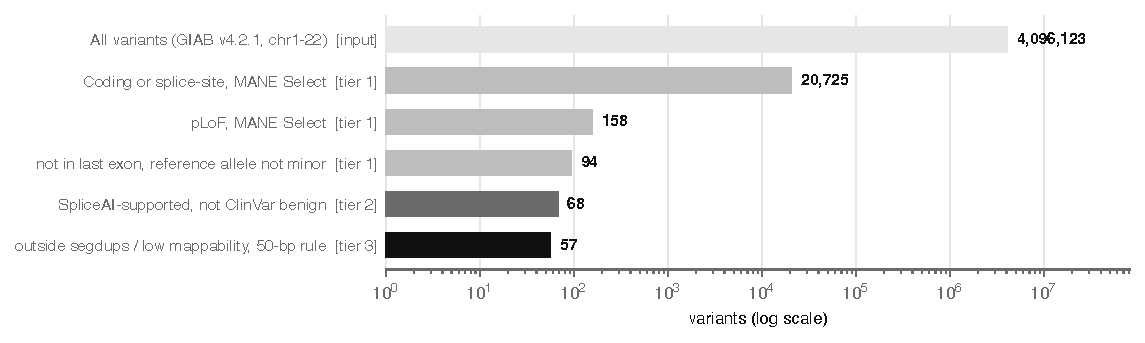
\includegraphics[width=0.85\textwidth]{figures/figS_funnel.pdf}
\caption{Variants of HG002 retained at each step. The pLoF steps count
variants with at least one MANE Select pLoF consequence that passes the
filters of the tiers applied so far (log scale; shading by tier).}
\label{fig:funnel}
\end{figure}

\begin{table}[ht]
\centering\small
\begin{tabular}{llp{0.42\textwidth}r}
\toprule
Tier & Flag & Source & Variants \\
\midrule
1 & last exon & \texttt{EXON} of the MANE Select consequence & \FlagLastExon{} \\
1 & allele frequency $\geq$ 95\% & gnomAD exomes/genomes in the core cache & \FlagRefMinor{} \\
2 & no SpliceAI support & SpliceAI plugin, all delta scores $<$ 0.2 & \FlagSpliceai{} \\
2 & ClinVar benign & ClinVar plugin, (likely) benign, not pathogenic & \FlagClinvarBenign{} \\
3 & 50-bp rule & Ensembl~116 GFF3 exon coordinates & \FlagFiftybp{} \\
3 & segmental duplication & GIAB v3.6 BED, \texttt{overlap()} & \FlagSegdup{} \\
3 & low mappability & GIAB v3.6 BED, \texttt{overlap()} & \FlagLowmap{} \\
\bottomrule
\end{tabular}
\caption{Flags applied to the \NPlof{} pLoF variants. A variant can carry
several flags; \NFlagged{} carry at least one.}
\label{tab:lofflags}
\end{table}

\subsection{Selection against loss of function in a single genome}
Genes intolerant to LoF were taken from the gnomAD v4.1 LOEUF metric; the
two lowest deciles contain the 20\% most constrained genes. Because longer
genes, which are more often constrained, carry more variants, rare
synonymous variants of HG002 serve as the reference: \LoeufSynPct\% of
them fall in the two lowest deciles. pLoF variants are depleted from these
genes (\LoeufAllPlofPct\%; odds ratio \LoeufAllPlofOr, Fisher's exact test
$p=\LoeufAllPlofP$), and their share generally increases towards the most
tolerant genes (Figure~\ref{fig:loeuf}). None of the \LoeufHcRareN{} rare
high-confidence pLoF variants with a LOEUF value lies in the two lowest
deciles. Rare missense variants are depleted to a lesser extent
(\LoeufAmLbPct\% for those AlphaMissense predicts as likely benign,
\LoeufAmLpPct\% for likely pathogenic; Table~\ref{tab:loeuf}).

\begin{figure}[ht]
\centering
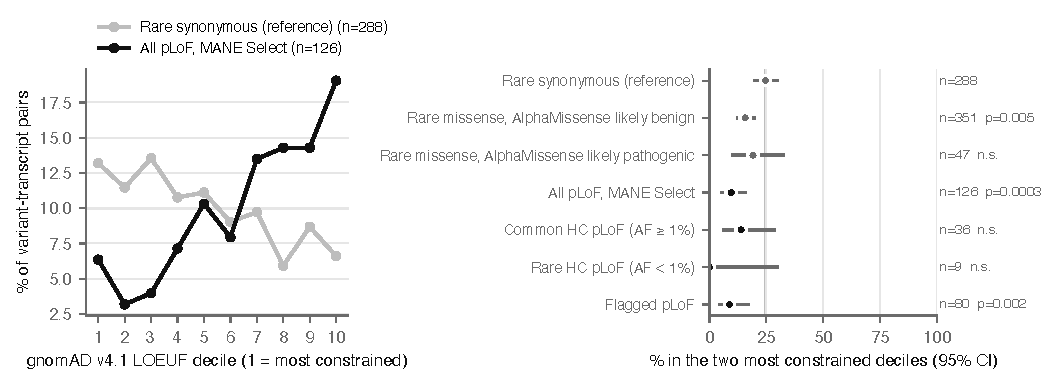
\includegraphics[width=\textwidth]{figures/figS_loeuf.pdf}
\caption{Variant classes of HG002 across gnomAD v4.1 LOEUF deciles. Left:
distribution of all MANE Select pLoF variants and of rare synonymous
variants. Right: share in the two most constrained deciles with 95\%
Wilson intervals; $p$-values from Fisher's exact test against rare
synonymous variants. Units are variant--transcript pairs in MANE Select
transcripts with a LOEUF value.}
\label{fig:loeuf}
\end{figure}

\begin{table}[ht]
\centering\small
\begin{tabular}{lrrrrr}
\toprule
Variant class & $n$ & Deciles 1--2 (\%) & Odds ratio & $p$ & Median LOEUF \\
\midrule
Rare synonymous (reference) & \LoeufSynN & \LoeufSynPct & -- & -- & \LoeufSynMedian \\
Rare missense, AM likely benign & \LoeufAmLbN & \LoeufAmLbPct & \LoeufAmLbOr & $\LoeufAmLbP$ & \LoeufAmLbMedian \\
Rare missense, AM likely pathogenic & \LoeufAmLpN & \LoeufAmLpPct & \LoeufAmLpOr & $\LoeufAmLpP$ & \LoeufAmLpMedian \\
All pLoF, MANE Select & \LoeufAllPlofN & \LoeufAllPlofPct & \LoeufAllPlofOr & $\LoeufAllPlofP$ & \LoeufAllPlofMedian \\
High-confidence pLoF, AF $\geq$ 1\% & \LoeufHcCommonN & \LoeufHcCommonPct & \LoeufHcCommonOr & $\LoeufHcCommonP$ & \LoeufHcCommonMedian \\
High-confidence pLoF, AF $<$ 1\% & \LoeufHcRareN & \LoeufHcRarePct & \LoeufHcRareOr & $\LoeufHcRareP$ & \LoeufHcRareMedian \\
Flagged pLoF & \LoeufFlaggedN & \LoeufFlaggedPct & \LoeufFlaggedOr & $\LoeufFlaggedP$ & \LoeufFlaggedMedian \\
\bottomrule
\end{tabular}
\caption{Share of each variant class in the two most LoF-intolerant LOEUF
deciles. AM, AlphaMissense; odds ratios and Fisher's exact test against rare
synonymous variants.}
\label{tab:loeuf}
\end{table}

\subsection{Clinically classified variants and their parental origin}
A single HG002 variant has a pathogenic or likely pathogenic ClinVar
classification with at least one review star:
\textit{\PlpGene} \PlpHgvsp{} (Table~\ref{tab:rarelof}), the factor~XI
``type~II'' allele (Glu117Ter in the legacy numbering of the mature
protein), heterozygous and inherited from the \PlpParent{}. Its gnomAD
frequency is \PlpAf\% overall but \PlpAsj\% in the Ashkenazi Jewish samples,
\PlpFold-fold higher, consistent with its known founder origin and with the
ancestry of the trio. Founder effects affect the rare pLoF variants more
generally: \NRareAsjCommon{} of the \NHcRare{} variants that are rare in
gnomAD overall have a frequency of at least 1\% in the Ashkenazi Jewish
samples. ClinGen curates \textit{F11} as semidominant; the variant would
therefore be reported as a carrier finding with possible partial factor~XI
deficiency, which this analysis does not assess.

Streaming the parental benchmark VCFs from S3 and the parental benchmark
regions over HTTPS resolves the origin of 9 of the 10 rare high-confidence
pLoF variants (\NRareMaternal{} maternal, \NRarePaternal{} paternal, one
homozygous variant carried by both parents); none is a candidate
\emph{de novo} variant. The unresolved variant, a 168-bp deletion in
\textit{HLA-DQB1}, lies outside the parental benchmark regions. The
homozygous variant illustrates a limit of transcript-level LoF calling: a
45-bp deletion that removes the canonical exon~2 splice donor of the MANE
Select transcript of \textit{PEX5}, whose biallelic loss of function causes
Zellweger spectrum disorder. The same exon has an alternative donor 45\,bp
downstream, and transcripts using it are annotated with an in-frame deletion.
Both parents are homozygous for the deletion, which is absent from gnomAD
and has conflicting classifications in ClinVar; the absence from gnomAD
reflects the length of the deletion rather than its rarity, and the variant
is most probably not a loss of function.

\begin{table}[ht]
\centering\scriptsize\setlength{\tabcolsep}{3pt}
\begin{tabular}{llp{0.2\textwidth}lllllll}
\toprule
Gene & Position & HGVS & Consequence & GT & AF & ASJ AF & ClinVar & MOI & Origin \\
\midrule
\tabinput{results/tex/tab_hc_rare.tex}
\bottomrule
\end{tabular}
\caption{Rare (gnomAD AF $<$ 1\%) high-confidence pLoF variants of HG002.
AF: maximum of the gnomAD exome and genome frequencies; ASJ AF: Ashkenazi
Jewish samples; MOI: ClinGen mode of inheritance (Moderate or stronger
gene--disease validity; SD, semidominant); origin from the parental
benchmark VCFs.}
\label{tab:rarelof}
\end{table}

\subsection{Callability of clinically relevant genes}
A negative result is informative only where the genome has been assessed.
\texttt{coverage()} of the MANE Select coding sequence by the HG002
benchmark regions shows that \NManeGenesLtNinety{} of \NManeGenes{} genes
and \NClinGenLtNinety{} of the \NClinGenGenes{} genes with a ClinGen
gene--disease relationship of at least moderate strength have less than 90\%
of their coding sequence in the benchmark (\NClinGenLtFifty{} less than 50\%;
Figure~\ref{fig:callability}, Table~\ref{tab:callability}). For
\NClinGenLtNinetyDifficult{} of these genes, most of the coding sequence lies
in GIAB difficult regions, such as segmental duplications, tandem repeats
or extreme GC content. \ClinGenFalseDup{} overlap regions that are falsely
duplicated in GRCh38; \textit{CBS}, the gene of classic homocystinuria, has
39\% of its coding sequence in the benchmark.

\begin{figure}[ht]
\centering
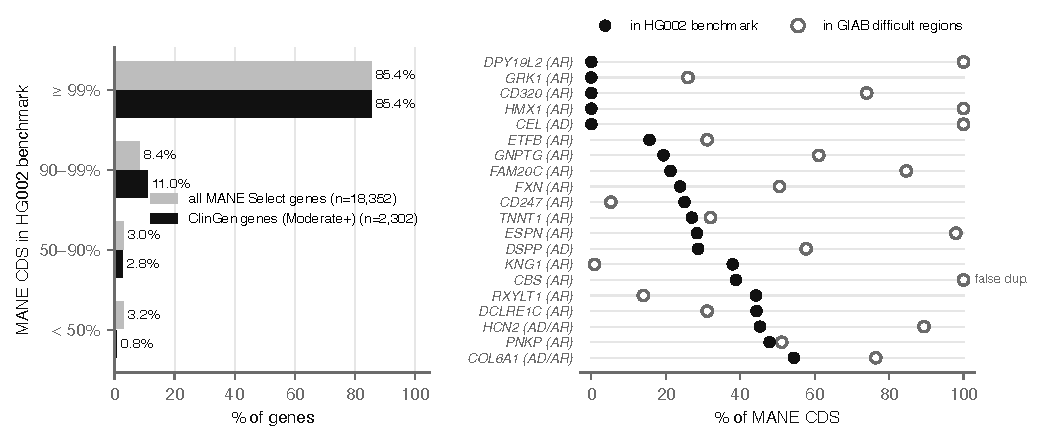
\includegraphics[width=\textwidth]{figures/figS_callability.pdf}
\caption{Share of the MANE Select coding sequence within the HG002 v4.2.1
benchmark regions. Left: genes binned by that share. Right: the 20 least
callable ClinGen genes, with the share of their coding sequence in GIAB
difficult regions (union of all v3.6 stratifications).}
\label{fig:callability}
\end{figure}

\begin{table}[ht]
\centering\scriptsize\setlength{\tabcolsep}{4pt}
\begin{tabular}{lrrrrll}
\toprule
Gene & CDS (bp) & Benchmark (\%) & Segdup (\%) & Difficult (\%) & MOI & Disease (ClinGen) \\
\midrule
\tabinput{results/tex/tab_callability.tex}
\bottomrule
\end{tabular}
\caption{The 25 ClinGen genes with the smallest share of MANE Select coding
sequence in the HG002 benchmark regions.}
\label{tab:callability}
\end{table}

\FloatBarrier
\subsection{Run time}
Annotation of the \NVariants{} variants with the core cache and four plugin
caches took \AnnotateSec\,s with \Workers{} workers; the remaining analysis,
including reading the \NRemoteSources{} ad hoc sources (\RemoteRows{}
million records in total) from their URLs in \RemoteSec\,s, took
\AnalyzeMin\,min, in a single Python process without intermediate VCF, BED
or index files. The tier-3 sources were not converted into caches: a change
of the question (another gene set, another stratification, another relative)
changes only the URL.

\subsection{Conclusions}
The example uses each tier for what it does best. The core cache supplies
VEP-identical consequences and population frequencies for 4.1 million
variants in minutes; plugin caches add frequently updated or licensed
evidence without rebuilding the core; and ad hoc sources answer
analysis-specific questions---gene constraint, curated disease genes, gene
models, genome stratifications and parental genotypes---through joins and
interval operations on the annotated frame. Biologically, the single genome
reproduces the depletion of LoF variants from constrained genes, recovers
the Ashkenazi founder allele \textit{F11} \PlpHgvsp{} with its parental
origin, and identifies the clinically relevant genes in which a negative
result would not be informative.



%% ===================================================================
\clearpage
\section{Notes on the analysis}
\label{sec:notes}
\destnone{Observations made while preparing the analysis, including
issues in polars-bio that affect claims about remote data.}
\begin{enumerate}
\item \textbf{polars-bio and HTTP(S) sources.} With polars-bio~\PolarsBioVersion{},
  \texttt{scan\_bed()} reads BED files over HTTPS, but \texttt{scan\_vcf()} and
  \texttt{scan\_gff()} abort on an \texttt{https://} path with
  ``\texttt{PanicException:} \texttt{not implemented:} \texttt{Unsupported storage type: HTTP}'' 
  (\nolinkurl{bio-format-vcf/src/physical_exec.rs:2719},
  \nolinkurl{bio-format-gff/src/physical_exec.rs:1244}); the VCF and GFF
  dispatchers handle only local files and GCS/S3/Azure object stores. The
  analysis therefore reads the parental VCFs from the GIAB mirror on S3
  (\texttt{s3://giab/\ldots}, anonymous access) and the Ensembl GFF3 with
  \texttt{polars.read\_csv()}. If the paper states that polars-bio reads
  remote genomic files ``by URL'', HTTP(S) support for VCF and GFF in
  datafusion-bio-formats should land first; the panic should in any case
  become a Python exception.
\item \textbf{Region pushdown on remote VCF.} A
  \texttt{chrom}/\texttt{start} filter on the S3 VCF (indexed with
  \texttt{.tbi}) took as long as a full scan (about 110\,s for 4.0 million
  records from Warsaw to \texttt{us-east-1}), i.e.\ the index is not used for
  remote files. The analysis streams each parental VCF once and joins it to
  the candidate variants instead.
\item \textbf{Live sources.} The ClinGen gene--disease validity file is
  regenerated daily (the copy used here was read on \today); for the
  published version, record its creation date and checksum, or pin a snapshot.
  gnomAD v4.1, GIAB v3.6/v4.2.1 and Ensembl~116 are versioned releases.
\item \textbf{Scope of the LoF filters.} The filters are modelled on LOFTEE
  (last exon, 50-bp rule, splice-site support) but are not LOFTEE: ancestral
  alleles, GERP, non-canonical splice motifs and the LOFTEE flags are not
  reproduced, and the published SpliceAI cache holds masked SNV scores only,
  so splice-site indels are not checked by SpliceAI. The wording in the paper
  should remain ``LOFTEE-inspired'' or name the filters explicitly.
\item \textbf{Benchmark regions.} The GIAB v4.2.1 benchmark covers chromosomes
  1--22 and excludes many difficult regions, so all counts are restricted to
  the benchmark and are lower bounds for the whole genome; the callability
  analysis quantifies this per gene. The newer HG002 Q100/T2T-based
  benchmark would extend coverage, but would need a GRCh38 liftover policy.
\item \textbf{Reporting findings in a named genome.} HG002 (PGP participant,
  open consent) is used in many publications; findings are reported here as
  ClinVar assertions and population frequencies only, without clinical
  interpretation. A sentence to that effect may be appropriate in the
  supplement.
\item \textbf{Environment.} The analysis used a clean environment with the
  PyPI releases vepyr~\VepyrVersion{}, Polars~\PolarsVersion{} and
  polars-bio~\PolarsBioVersion{}; the repository development
  \texttt{.venv} on the authoring machine still has polars-bio~0.26.0 and a
  stale native module (\texttt{import vepyr} fails there).
\item \textbf{References.} The bibliography of this document was written
  from memory for the draft; verify each entry (volume, pages, year) before
  adding the keys to \texttt{references.bib}.
\item \textbf{Haplotype-aware consequences.} The compensating frameshift
  pairs in \textit{SON} and \textit{SLAIN1} are annotated as two
  frameshifts because VEP (and vepyr) annotate each allele separately; the
  frequency filter catches them here, but a haplotype-aware consequence mode
  would be the principled fix.
\end{enumerate}


\begin{thebibliography}{99}\small
\bibitem{aganezov2022} Aganezov S, et al. A complete reference genome improves analysis of human genetic variation. \emph{Science} 376:eabl3533 (2022).
\bibitem{asakai1991} Asakai R, Chung DW, Davie EW, Seligsohn U. Factor XI deficiency in Ashkenazi Jews in Israel. \emph{N Engl J Med} 325:153--158 (1991).
\bibitem{cheng2023} Cheng J, et al. Accurate proteome-wide missense variant effect prediction with AlphaMissense. \emph{Science} 381:eadg7492 (2023).
\bibitem{dolphin1998} Dolphin CT, et al. The flavin-containing monooxygenase 2 gene (FMO2) of humans, but not of other primates, encodes a truncated, nonfunctional protein. \emph{J Biol Chem} 273:30599--30607 (1998).
\bibitem{dwarshuis2024} Dwarshuis N, et al. The GIAB genomic stratifications resource for human reference genomes. \emph{Nat Commun} 15:9029 (2024).
\bibitem{jaganathan2019} Jaganathan K, et al. Predicting splicing from primary sequence with deep learning. \emph{Cell} 176:535--548 (2019).
\bibitem{karczewski2020} Karczewski KJ, et al. The mutational constraint spectrum quantified from variation in 141,456 humans. \emph{Nature} 581:434--443 (2020).
\bibitem{macarthur2012} MacArthur DG, et al. A systematic survey of loss-of-function variants in human protein-coding genes. \emph{Science} 335:823--828 (2012).
\bibitem{morales2022} Morales J, et al. A joint NCBI and EMBL-EBI transcript set for clinical genomics and research. \emph{Nature} 604:310--315 (2022).
\bibitem{rip2006} Rip J, et al. Lipoprotein lipase S447X: a naturally occurring gain-of-function mutation. \emph{Arterioscler Thromb Vasc Biol} 26:1236--1245 (2006).
\bibitem{strande2017} Strande NT, et al. Evaluating the clinical validity of gene--disease associations. \emph{Am J Hum Genet} 100:895--906 (2017).
\bibitem{wagner2022} Wagner J, et al. Benchmarking challenging small variants with linked and long reads. \emph{Cell Genomics} 2:100128 (2022).
\bibitem{zook2016} Zook JM, et al. Extensive sequencing of seven human genomes to characterize benchmark reference materials. \emph{Sci Data} 3:160025 (2016).
\end{thebibliography}

\end{document}
